Obvious is a set of interfaces and extension classes for wrapping
around existing information visualization toolkits.  It generalizes
and extends the standard architecture as defined in the Information
Visualization reference model to try to abstract all the existing
implementations.  In this section, we list some major existing
toolkits and explain what they share and how they differ.  In the
second section, we describe the most common standardization processes
for software systems.

\subsection{Visualization Toolkits}

Pretty much all existing information visualization toolkits follow the
InfoVis reference model initially specified by Ed Chi and refined by
Card, Mackinlay and Shneiderman~\cite{ChiRefModel,ReadingsIV} and has
been described as a design pattern in~\cite{DesignPatternsIV}.  The
model defines three stages: \emph{DataSet} or \emph{Data Tables},
\emph{Visualization} or \emph{Visual Structure} and \emph{View}
(Figure~\ref{fig:refmodel}).  One of its main benefits is that it
explicitly represents interaction, in contrast to older visualization
models.  Several articles have described the concrete design of an
information visualization toolkit.  We report here on the common and
the specific parts.

\begin{figure}
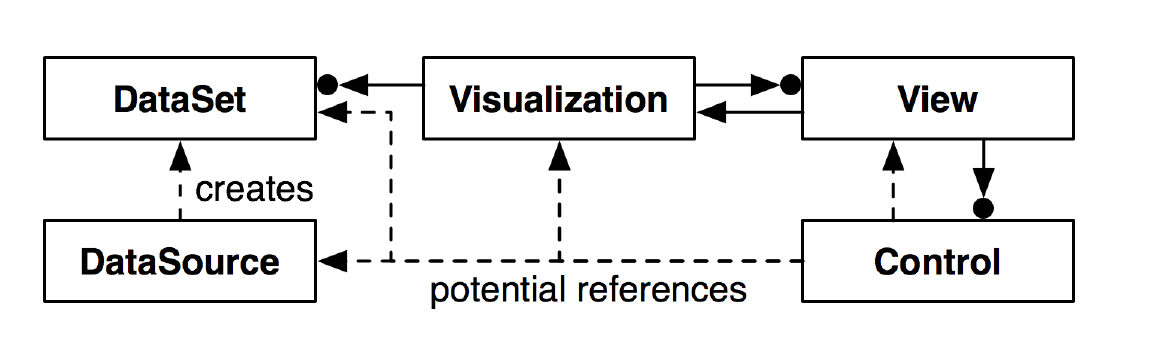
\includegraphics[width=\columnwidth]{figures/refmodpat}
\caption{The Information Visualization Reference Model~\cite{DesignPatternsIV}}
\label{fig:refmodel}
\end{figure}


The InfoVis Toolkit~\cite{InfoVis} is based on an \emph{in-memory
  database manager} where data is organized in columns --- contrary to
most persistent relational databases --- to improve the memory
footprint and allow addition of new attributes that are needed to
manage the interaction (e.g. selection or filtering) and to hold
attributes computed on demand.  The main challenge being the support
of interactive performance for rendering and dynamic queries with a
small memory footprint.  The visual structure is managed using a
\emph{monolithic} architecture~\cite{Polylithic}: each visualization
technique is implemented as a specific class
(e.g. ScatterplotVisualization, ParallelCoordinatesVisualization,
TreeVisualization) that performs the mapping between the data set and
the graphics items to render.  Finally, the view component is the same
for each of the visual structures and takes care of scrolling,
zooming, overlaying magic lenses (e.g. Fisheye or Magic Lenses).  A
\emph{notification mechanism} implements the communication between the
data tables and the visual structure: each time a data table is
modified, it notifies all the registered handlers of the details of
the modification. The interaction is managed by \emph{Interactor}
objects that are associated with the visual structures; the views are
generic and forward interaction managements to the Interactors.  One
specific feature provided by the InfoVis Toolkit is layering:
visualization can be composed on top of each others.  Composite
visualizations are useful to build complex visualization by breaking
them into simple parts. For example, node-link diagrams are split into
links managed as a layer and nodes as another.  Magic lenses and
Fisheyes are also managed as layers on top of other visualizations.

Prefuse~\cite{Prefuse} also relies on an in-memory database with
notification but implements the visual structure using an extension of
the data model (a visual table derives from a data table).  It then
transforms the data into a \emph{polylithic} graphic structures
whereas all the other toolkits use a \emph{monolithic} architecture.
In a polylithic architecture, there is only one component in charge of
all the visual structures.  A visualization object is responsible of
managing a visual structure: it contains visual tables that augment
data tables with graphic attributes (shape, color, etc.)
Visualizations are in charge of computing the layout (assigning a
position and shape to visual items), the graphic attributes and
animations.  Visualizations use a \emph{Renderer} object to actually
display visual items.  Users can control which renderer is used
depending on the visualization and the object itself.  In Prefuse,
data managers, visual managers and views are generic, offering a very
clean interface to the application programmer.  However, as noted by
Bederson at al.~\cite{Polylithic}, polylithic toolkits have a steeper
learning curve than monolithic ones because the polylithic components
do not work out of the box, they always need to be configured.  To
address this issue, Prefuse comes with code samples that simplify the
initial setup.

Building upon their experience in the Prefuse toolkit~\cite{Prefuse},
Heer et Agrawala~\cite{DesignPatternsIV} have derived software design
patterns that are common to information visualization applications and
toolkits. 

Improvise~\cite{Improvise} relies on an in-memory database with
notification that is row-oriented and its visual structures are
monolithic.  The main characteristic of Improvise lies in its
management of coordinated views.  To this aim, it relies on several
design patterns not supported by Prefuse; compared to the other
information visualization toolkits, it adds a coordination component
that is central and extends the notification mechanism implemented
by the InfoVis Toolkit or Prefuse.

Discovery~\cite{Discovery1,Discovery2,Discovery3} shares most of its
characteristics with Prefuse: it uses an in-memory, column-oriented
database and a polylithic graphic model. Its two main features are 1)
the absence of a scene graph, replaced by a dataflow pipeline made of
short operations called \emph{functors} that renders directly from the
data-model, and 2) a deferred notification strategy to allow data
editing.

%% \jo{I'm not sure I am convinced of the assertion in the following
%%   paragraph. The three toolkits above are described in some detail,
%%   not all of which is relevant to other toolkits. Perhaps we should
%%   instead abstract their distinct design characters. e.g. Row-oriented
%%   vs column oriented; in-memory vs cached database management;
%%   monolithic vs polylithic etc. The point being that while they all
%%   attempt to achieve similar general aims, their lower-level approach
%%   to doing so requires different programming approaches, hence the
%%   need for Obvious.}

Other information visualization toolkits can mostly be described using
the four toolkits above, even if they use a different programming
language.  Tulip~\cite{Tulip} is a graph-oriented toolkit programmed
in C++ that uses data tables for vertices and edges, like the InfoVis
Toolkit and Prefuse.  It implements several complex graph layout
algorithms and uses OpenGL for its rendering but the conceptual
architecture is table-based and monolithic.  Therefore, information
visualization toolkits share a global organization, they all implement
an in-memory database with two variants (row-based or column-based), a
visual structure with two variants (monolithic or polylithic) and
several specific features.  Even if some choices made by toolkits
designers were carefully decided, other were probably made without
being aware of the alternatives.  Combining the best possible features
for a next-generation toolkit might be tempting but there are still
tradeoffs that cannot be solved.  For example, the power of
coordinated and linked views offered by Improvise comes at the cost of
maintaining caches that should be flushed when the data change so
there seems to be a tradeoff there that still needs research to be
solved.

There are also lower-level toolkits that can be used to build visual
analytics applications.  Two popular families are graphics libraries
and graph libraries.

%% \jo{I'm not sure what point is being made here with the discussion of
%%   lower level visualization toolkits. Are we asserting that the
%%   standardization implied by Obvious is also appropriate for lower
%%   level approaches to VA software construction? If so, we need to
%%   identify what is lacking in an approach without Obvious as well as
%%   demonstrating (later on in the paper) that implementing the Obvious
%%   interfaces in lower level visualization environments is both
%%   practical and beneficial. An interesting test case might be
%%   \emph{Processing} (processing.org). This is, compared to the other
%%   examples cited, a very low level approach to visualization software
%%   development. However, it is designed for rapid-prototyping, and if
%%   it could be easily integrated with Obvious it might provide a nice
%%   example of how early prototypes could be transformed into more
%%   robust applications using Obvious as the bridge. I'd be happy to
%%   write some words on this if you think it fits well with the theme of
%%   the paper.}

\subsection{Graphics Libraries}

Visual analytics applications can manage their own data structure and
take care of the mapping from data to visualization on their own.  At
this point, they can use \emph{scene-graphs} or \emph{direct-graphics}
libraries.  

Scene-Graph toolkits can manage the visual structure and view as
described in the reference model.  They are focused on computer
graphics and interaction: they only deal with the visual structure and
view.  Piccolo and Jazz~\cite{Polylithic} are popular 2D scene-graph
managers that have been used to create several information
visualization applications (e.g.~\cite{SpaceTree,Geneaquilt}.) An
early version of Piccolo has also been used as graphics engine for the
Cytoscape graph visualization system~\cite{Cytoscape} but dropped for
performance reasons.

High-performance information visualization applications use
scene-graph optimization techniques to speed-up the rendering of
scenes.  Tulip~\cite{Tulip} and Gephi~\cite{Gephi} maintain a spatial
indexing structure to avoid rendering objects that are not visible.

Although scene-graph technologies are mature and used in a wide
variety of graphics applications such as games, virtual-reality
applications and scientific visualization systems, they are not always
adequate for information visualization systems because they require
the explicit specification of geometry and graphic attributes for each
displayed objects.  Very often, information visualization can quickly
compute graphic attributes and even geometry from data attributes.
For example, the position of an item using a scatterplot visualization
is computed using a simple affine transformation the data attributes
using for the X and Y dimensions.  There is no need to store the
computed values when computing them on the fly is very cheap.  The
same is true for color etc.  Copying and storing this information is
costly in terms of time and memory.

Direct-graphics libraries such as \emph{Processing} or \emph{OpenGL}
can also be used to implement the visualization technique while
drawing for rapid prototyping or high-performance reasons.

[Add a section on Processing]

Still, when separating the data-model from the visual model,
scene-graph managers offer more flexibility than information
visualization systems for complex graphics and sophisticated
interaction.  This is why several information visualization systems
still use them.

% say something about the fact that scene-graph toolkits are
% classically for 3D scenes.

\subsection{Graph Libraries}

While most table-based visualization toolkits rely on an in-memory
database, several graph-based visualization systems manage their
data-structures using a model inspired from graph-theory where
topology is the main focus and data associated with graph entities is
less important.  This is the case for the JUNG library~\cite{jung2003}
or the Boost Graph Library (BGL)~\cite{BGL}, as well as for the graph
library used by Cytoscape~\cite{Cytoscape}.

These libraries support graphs as set of vertices and edges (the
topological entities) that can be associated with arbitrary data.
This data is just stored by the graph entities as a convenience for
the application: the library does not implement any integrity check
between data and graph entities.  In contrast, the InfoVis Toolkit,
Prefuse and Tulip maintain a close consistency between graphs and data
tables: removing a data table entry associated with a graph entity
(vertex or edge) also removes the entity from the graph structure.

Thus, there is no clear consensus on how a graph data structure should
be managed internally; the design choices are quite different
depending on the communities such as graph theory, information
visualization, database and semantic web.


\subsection{Standardization Processes}

Standardization is a well established habit in the software community;
several standardization models have been used in the past and these
models tend to evolve due to the growing pace of software development
taking place nowadays.

Standards have been specified by national and international
organization such as the International Organization for
Standardization (e.g. ISO, ASCII), non-profit organizations (e.g. the
Unicode Consortium or OMG), consortia of public or private
organizations (e.g. the World Wide Web Consortium (W3C)). Closer to
the information visualization community, ``The Open Geospatial
Consortium (OGC)\footnote{\url{http://www.opengeospatial.org}} is an
international industry consortium of 423 companies, government
agencies and universities participating in a consensus process to
develop publicly available interface standards.''

\jdf{More to come..}
